\chapter{Complex event processing}
	\label{chap:cep}
	\section{Intro of the Complex Event Processing}
		In this hierarchical runtime verification project, the top level of modelling is done in an event pattern language.
		This event pattern language is translated to timed event automatons. These event automatons will be executed in the
		process.
	\section{Formal Intro of the Timed Parametrized Event Automaton}
		\subsection{VEPL}
			Our choice for the event pattern definition is the VIATRA Event Pattern Language (VEPL).
			Currently this is the only CEP which can be easily integrated to a live model, where 
			you can define multiple graph patterns over the model, and define atomic events for the
			appearance and disappearance of these patterns.
			
			TODO define complex event processing
			
			A brief overview of the VEPL language:

		\begin{tabular}{lcm{6cm}}
		\centering
		Operator name &	Denotation & Meaning \\
		followed by & p1 $\rightarrow$ p2 & Both patterns have to appear in the specified order. \\
		or &	p1 OR p2 &	One of the patterns has to appear. \\
		and &	p1 AND p2 &	Both of the patterns has to appear, but the order does not matter. Rule: p1 AND p2 $\equiv$ ((p1 $\rightarrow$ p2) OR (p2 $\rightarrow$ p1)). \\
		negation &	NOT p &	On atomic pattern: event instance with the given type must not occur. On complex pattern: the pattern must not match. \\
		multiplicity &	p\{n\} &	The pattern has to appear n times, where n is a positive integer. Rule: p\{n\} $\equiv$ p1 $\rightarrow$ p1 $\rightarrow$ \dots p1, n times. \\
		"at least once" multiplicity &	p\{+\} &	The pattern has to appear at least once. \\
		"infinite" multiplicity &	p\{*\} &	The pattern can appear 0 to infinite times. \\
		within timewindow &	p[t] &	Once the first element of the pattern is observed (i.e. the patterns ``starts to build up''), the rest of the pattern has to be observed within t milliseconds.
		\end{tabular}	
			
			%% Regular -> Timed Regular -> Event Automata (parametrized) -> MERGE -> Timed Event Automaton
		\subsection{Timed Regular Expression}
			\begin{dfn}
				Timed Regular Expressions over an alphabet $\Sigma$ (also referred to as $\Sigma$-expressions)
				are defined using the following families of rules~\citep{tre}~.
				\begin{enumerate}
					\item \underline{a} for every letter $a \in \Sigma$ and the special symbol $\varepsilon$ are expressions.
					\item If $\varphi, \varphi_1, \varphi_2$ are $\Sigma$-expressions and $I$ is an integer-bounded interval then
						$\langle\varphi_I\rangle, \varphi_1~\cdot~\varphi_2, \varphi_1 \vee \varphi_2,$ and $\varphi^\ast$ are $\Sigma$-expressions.
					\item If $\varphi, \varphi_1$ and $\varphi_2$ are $\Sigma$-expressions then $\varphi_1 \circ \varphi_2, \varphi^\circledast$ are
						$\Sigma$-expressions.
					\item If $\varphi_1$ and $\varphi_2$ are $\Sigma$-expressions, $\varphi_0$ is a $\Sigma_0$-expression
						for some alphabet $\Sigma_0$, and $\Theta$ : $\Sigma_0 \rightarrow \Sigma$ is
						a renaming, then $\varphi_1 \wedge \varphi_2$ and $\Theta(\varphi_0)$ are $\Sigma$-expressions.
				\end{enumerate}
			\end{dfn}
			
		\subsection{Event Automaton Formalisms}
			\begin{dfn}
				\label{dfn:cep:dfea}
				A EventAutomaton (Deterministic Finite Event Automaton in other words) $\langle Q,\Sigma,\delta_d,q_0, F \rangle$ tuple where: %TODO Deterministic
					\begin{itemize}
						\item $Q$ is a finite, non empty set. These are the states of the automaton,
						\item $\Sigma$ is a finite, non empty set. This is the Event set of the automaton,
						\item $\delta_d$ is a set of $\langle Q \times \Sigma \times Q \rangle$ tuples,
							and the number of outgoing edges from each state for each event is only one 
							i.e. $\forall q_0 \in Q$ and $\forall e_0 \in \Sigma$ : $|\langle q_0, e_0, q_1 \rangle| = 1$, where $q_1 \in Q$ 
						\item $q_0 \in Q$ a start state,
						\item $F \subseteq Q$ the set of the acceptor states.
					\end{itemize}
				
			\end{dfn}
			
			In simulation we can define tokens. Somehow. Not now. %%TODO
			
			
			On input $e$, where $e \in \Sigma$, if the token is on State $s$ the next state will be $s'$ where 
			$\delta_d \langle s,e,s' \rangle$ 
			
			% \begin{dfn}
				% NonDeterministicTimedFiniteAutomaton
				% $\delta = \delta_t \cup \delta_d$ where $\delta_d$ is the same as $\delta$ in Definition \cite{dfn:cep:fsm}
				% $t$ is a clock variable $t \in R$   %todo R  
				% $\Sigma_n = \Sigma \cup T$
				% where $\Sigma$ is the oldSigma and T is 
			% \end{dfn}
			
			% \begin{dfn}
				% \label{dfn:cep:nsm}
				% A NonDeterministicFiniteAutomaton $\langle Q,\Sigma,\delta,q_0, F \rangle$ where 
				% the meaning of $Q, \Sigma, q_0,$ and $F$ is the same as Definition \ref{dfn:cep:fsm},
				% except for for $\delta$ which is
					% \[ \delta(q,a) \subseteq Q \]
				% where $q \in Q$ and $a \in \Sigma \cup \{\varepsilon\}$
			% \end{dfn}
			
			\begin{dfn}
				A Timed Event Automaton $\langle Q,\Sigma,\delta,q_0, F, t, T \rangle$ where
				\begin{itemize}
					\item $Q, \Sigma, q_0,$ and $F$ are the same as in Definition \ref{dfn:cep:dfea},
					\item $t$ is a global clock variable $t \in \mathbb{R}$,
					\item $T$ is a set of tuples $\langle Q, \RR \rangle$
					\item and $\delta$ is the union of discrete and timed transitions i.e. $\delta_t \cup \delta_d$ where
					\begin{itemize}
						\item $\delta_d$ is defined as in Definition \ref{dfn:cep:dfea},
						\item and $\delta_t$ represents timed transitions and defined as the set of tuples $\langle Q \times \mathbb{R} \times Q \rangle$ 
					\end{itemize}
				\end{itemize}
				
				
			\end{dfn}

			The semantic of the Timed Nondeterministic Finite Automaton is defined as follows:
			$Q_t \subseteq Q$ is the set of states with outgoing timed transitions, i.e. $\forall s \in Q_t$ : there exist $ \delta_t\langle s, t, s' \rangle$ where $t \in \RR$ and $s' \in Q$.
			We have to define rules for entering states with timed outgoing transitions and we also define the general rules of changing states. 
			\begin{enumerate}
				\item Entering Timed State Rule: On entry to state $s$ where $s \in Q_t$ the timeout variable $t_s$ of the state is set according to the value of the global time and the timeout value of the output transition $t_{timeout}$:
					$t_s:= t+t_{timeout}$ %\TODO
					where $T\langle s,t_s \rangle$ and $\delta_t\langle s,t_{timeouts},s' \rangle$ where $t_{timeout}$ is minimal from the set of possible $t_{timeouts}$ 
				
				\item Firing Transitions Rule: Nondeterministically choose an enabled transition from the set of enabled discrete or timed transitions. We have two cases, the chosen transition is:
					\begin{enumerate}
						\item Discrete Transition: In case of $s \notin Q_t$ than the execution of the transition is as in described formerly. If we exit state $s \in Q_t$ by a transition in $\delta_d$, 
						then the following rule extends the firing rule of discrete transitions:
							$t_s := \infty$
						\item Timed Transition: The transition with the minimal timeout value is selected, i.e. transition $\delta_t$ from state $s_t$ where $\forall q \in Q_t: t_q \geq t_s$, than the following rules apply:
						 the global time is set $t := t_s$, the local clock is set to infinity: $t_s := \infty$ and move to the next state according to $\delta_t$.
							
					\end{enumerate}
					
					% \item \label{rule:cep:tndfa2} 
					% If a token enters $s_t$ where $s_t \in Q$ and $|\delta_t\langle s_t, i, s_j\rangle | > 0$ where $i \in \RR$ and $s_j \in Q$,
					% at time $t'$ where $t' = t + t_{min}$ where $t$ is the time of enter and $t_{min}$ is the minimum of the $i$'s then the token will be moved to $s_{destination}$ 
					% where $\delta_t \langle s_t,i_{min}, s_{destination} \rangle$ %refactor pls
					% \item If a token exits by rule \ref{rule:cep:tndfa2} $t := t'$
			
			\end{enumerate}
			
		\subsection{Extending the Event Automaton Formalism}
			
			We use $s$ to denote a tuple $\langle s_0,\dots,s_k \rangle$. We use $X \rightarrow Y$ and $\rightharpoondown$ to denote sets of total and partial function between
			$X$ and $Y$, respectively. We write maps (partian functions) as $[x_0 \mapsto v_0,\dots,x_i \mapsto v_i]$ and the empty maps as $[]$. Given two maps $A$ and $B$,
			the map override operator is defined as:
				\[
				 (A \dagger B)(x) = 
				  \begin{cases} 
				   B(x) & \text{if } x \in \text{\underline{dom}(B)} \\
				   A(x) & \text{if } x \notin \text{\underline{dom}(B)} \text{ and } x \in \text{\underline{dom}(A)} \\
				   \text{undefined otherwise.}
				  \end{cases}
				\]
 			
			\begin{dfn}
				(Smybols, Events, Alphabets and Traces).
				Let $\mathit{Sym} = \mathit{Val} \cup \mathit{Var}$ be the set of all symbols (variables or values).
				An event is a pair $\langle e, \overline{s} \rangle \in \Sigma \times \mathit{Sym}^\ast,$ written $e(\overline{s})$.
				An event $e(\overline{s})$ is ground if $\overline{s} \in \mathit{Val}^\ast$.
				Let Event be the set of all events and GEvent be the set of all ground events.
				A trace is a finite sequence of ground events.
				Let Trace = $GEvent^\ast$ be the set of all traces
			\end{dfn}
			
			\begin{dfn}
				(Substitution).
				The binding $\theta = [x_0 \mapsto v_0, \dots, x_i \mapsto v_i]$ can be applied to a symbol $s$ and to an event
				$e(\overline{s})$ as follows: 
				\[
				 s(\theta) = 
				  \begin{cases} 
				   \theta(s) & \text{if } s \in \underline{dom}(\theta) \\
				   s & \text{otherwise}
				  \end{cases}
				  \qquad e \langle s_0,\ldots,s_j \rangle (\theta) = e \langle s_0(\theta),\ldots,s_j(\theta) \rangle
				\]
			\end{dfn}
			
			\begin{dfn}
				(Matching).
				Given a ground event a an event b the predicate matches (a, b) hold if there exists a binding $\theta$ s.t. b($\theta$) = a.
				Moreover let match(a,b) denote the smallest such binding w.r.t $\sqsubseteq$ if it exists (and is undefined otherwise)
			\end{dfn}
			
			\begin{dfn}
				(Configurations and Transition Relation).
				We define configurations as elements o the set Config = Q $\times$ Bind. Let $\rightarrow \subseteq$ Config $\times$ GEvent $\times$ Config be a relation on
				configurations s.t. configurations $\langle q, \varphi \rangle$ and $\langle q', \varphi' \rangle$ are related by the ground event a, written
				$\langle q, \varphi \rangle \xrightarrow{\text{a}} \langle q' \varphi' \rangle$ if, and only if
					\begin{align}
						\exists b \in \mathcal{A}, \exists g \in &Guard, \exists \gamma \in Assign : (q, b, g, \gamma, q') \in \delta \wedge \\
						&matches(a,b) \wedge g(\varphi \dag match(a,b)) \wedge \varphi' = \gamma(\varphi \dagger match(a,b))
					\end{align}
				Let the transition relation $\rightarrow_{E}$ be the smallest relation containing $\rightarrow$ such that for any event
				$a$ and configuration $c$ if $\nexists c' : c \xrightarrow{\text{a}} c'$ then $ c \xrightarrow{\text{a}}_E c$.
				The relation $\rightarrow_E$ is lifted to traces.
				For any two configurations $c$ and $c'$, $ c \xrightarrow{\text{$\epsilon$}}_E c$ holds, and $\xrightarrow{\text{a.$\tau$}}_E c'$ holds
				if there exist a configuration $c'$ s.t. $c \xrightarrow{\text{a}}_E c'' \xrightarrow{\text{$\tau$}}_E c'$
			\end{dfn}
			
			
			
			
			
			We can extend the time behaviour from states to configurations(set of states). % TODO
			In this case :
				A timeout variable is set to configurations, not just states
				And if a token enters a configuration it sets the timer.
				We can either move with 
					discrete events the same as before
					or with timeout events (which are activated if there is a token in any of the states of the configuration)
				
			
			
			
			This generates a language \dots %%TODO
				
			In runtime verification this will accept \dots %%TODO
				
			
		
		% \subsection{Event Automaton}
			% % informal definition
			% An Event Automaton is a non-deterministic finite-state automaton whose alphabet consists
			% of parametric events and whose transitions may be labelled with guards and assignments
			
			% % formal definition
			% \begin{dfn}
				% An EA
				% $\langle Q,\mathcal{A},\delta, q_0, F \rangle$ is a tuple where Q is a finite set of states, 
				% $\mathcal{A} \subseteq Event$ is a finite alphabet,
				% $\delta \in (Q \times \mathcal{A} \times Assign \times Q)$ is a finite set of transitions, 
				% $q_0 \in Q$ is an initial state, and 
				% $F \subseteq Q$ is a set of final states\citep{qea}.
			% \end{dfn}
			
		% \subsection{Timed Event Automaton}
			% % stuff about the calendar
			% % informal definition of the calendar?
			% In discrete event simulation, a calendar (also called event list) is a data structure that
			% stores future events and the times at which these events are scheduled to occur
			
			% Formal definition of the calendar
				% \begin{dfn}
				% A calendar is a finite set (or multiset) of the form $C = \{ \langle e_1, t_1\rangle \, \dots ,\langle e_n, t_n\rangle \}$
				% where each $e_i$ is an event and $t_i$ is the time when event $e_i$ is scheduled to occur. All $t_i$s are real numbers.
				% We denote by min(C) the smallest number among $\{t_1,\dots ,t_n \}$ (with min(C) = $+\infty$ if C is empty)
				% Given a real u, we denote by $Ev_u(C)$ the subset of C that contains all events scheduled at time u:
				% $Ev_u(C) = \{ \langle e_i, t_i \rangle  | t_i = u \wedge \langle e_i , t_i \rangle \in C \} $
				% \end{dfn}
			% % stuff about the calender automaton
				
			% \begin{dfn}
				% A TimedZone $\langle S,\mathcal{E},I,T \rangle $ is a tuple where $S \in$ States,
				% $T \in$ States, 
				% $\mathcal{E}~\subseteq$~States,
				% $I$ is a time value 
			% \end{dfn}
			
			% The semantic of the TimedZone is the following: 
				% If a token enters state $S$ at $t_i$, and doesn't reach any of the $\mathcal{E}$ states before $t_j$,
				% where $t_j = t_i + I$, then the token is moved to $T$
				
			% \begin{dfn}
				% A TEA
				% $\langle E,\mathcal{T} \rangle$ is a tuple where $E$ is an Event Automaton, and $\mathcal{T}$ is a set of Timed Zones, where all the states are one of the 
				% Automatons states.
			% \end{dfn}

		\subsection{Compilation of the Event patterns to Parametrized Event Automata}
			
			
			
	\section{Examples of Event Processing}
 
		\subsection{Sequence chart example}
 
		\subsection{File System}
			\subsubsection{Problem}
				File system - A file shouldn't be read when it has been opened for writing, and shouldn't be written, when opened for reading. 
				A file shouldn't be opened for writing and reading without a close event between the two different opens~\citep{marq}.
				The possible parametrized events are : 
				Open(file, mode), 
				Close(file), 
				Read(file), 
				Write(file). 
				Mode is either "R" or "W" which stands for Read and Write respectively.
			\subsubsection{Solution}
				We are looking for these patterns :

				\begin{itemize}
					\item open(f,"W") $\rightarrow$ NOT close(f)$\{\ast\}$ $\rightarrow$ open(f,"R");
					\item open(f,"R") $\rightarrow$ NOT close(f)$\{\ast\}$ $\rightarrow$ open(f,"W");
					\item open(f,"W") $\rightarrow$ NOT close(f)$\{\ast\}$ $\rightarrow$ read(f);
					\item open(f,"R") $\rightarrow$ NOT close(f)$\{\ast\}$ $\rightarrow$ write(f);
				\end{itemize}

				These event patterns can be matched with the automaton seen on \cref{fig:cep:fileautomaton}
				
				\begin{figure}[h]
				\centering
				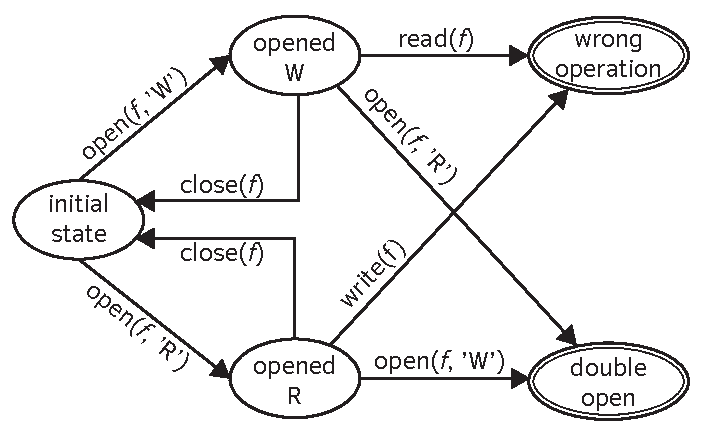
\includegraphics[width=0.7\linewidth]{include/figures/chapter_5/file_example_aut}
				\caption{Automaton of the file example}
				\label{fig:cep:fileautomaton}
				\end{figure}

		
		
		\subsection{Mars Rover Tasking - Two phase locking}
			\subsubsection{Problem}
				In concurrent systems the avoidance of deadlocks and livelocks are an utmost importance.
				To solve this problem, one of the many patterns is  the two phase locking - which can be defined by two rules.
				These rules are : 
				\begin{enumerate}
					\item \label{itm:cep:mp1} Every task must allocate the resources in a given order.
					\item \label{itm:cep:mp2} If a task releases a resource, it can't allocate anymore
				\end{enumerate}
			\subsubsection{Solution}
				Since our implementation doesn't support guards \emph{yet} we can only use constant amount of resources.
				For this example, this amount will be set to two, to minimise the model of the example.
				The \cref{itm:cep:mp1} pattern can be matched with the \cref {fig:cep:marsautomaton1}, and the \cref{itm:cep:mp2} 

				\begin{figure}[h]
				\centering
				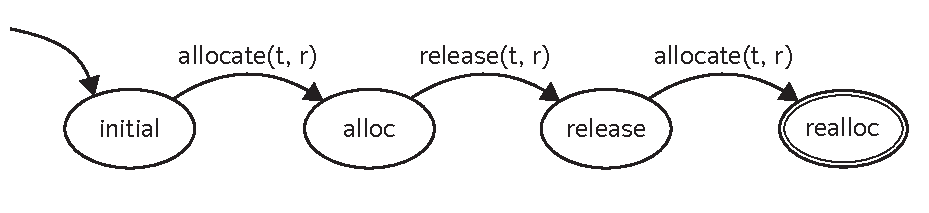
\includegraphics[width=0.7\linewidth]{include/figures/chapter_5/mars_example_aut1}
				\caption{Automaton to forbid the reallocation}
				\label{fig:cep:marsautomaton1}
				\end{figure}		
				
				
				\begin{figure}[h]
				\centering
				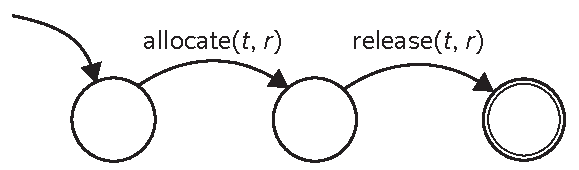
\includegraphics[width=0.7\linewidth]{include/figures/chapter_5/mars_example_aut2}
				\caption{Automaton to forbid inverse allocation}
				\label{fig:cep:marsautomaton2}
				\end{figure}	

				
				
	\section{Implementation}
		\subsection{Metamodel}
		
			\begin{figure}[h]
			\centering
			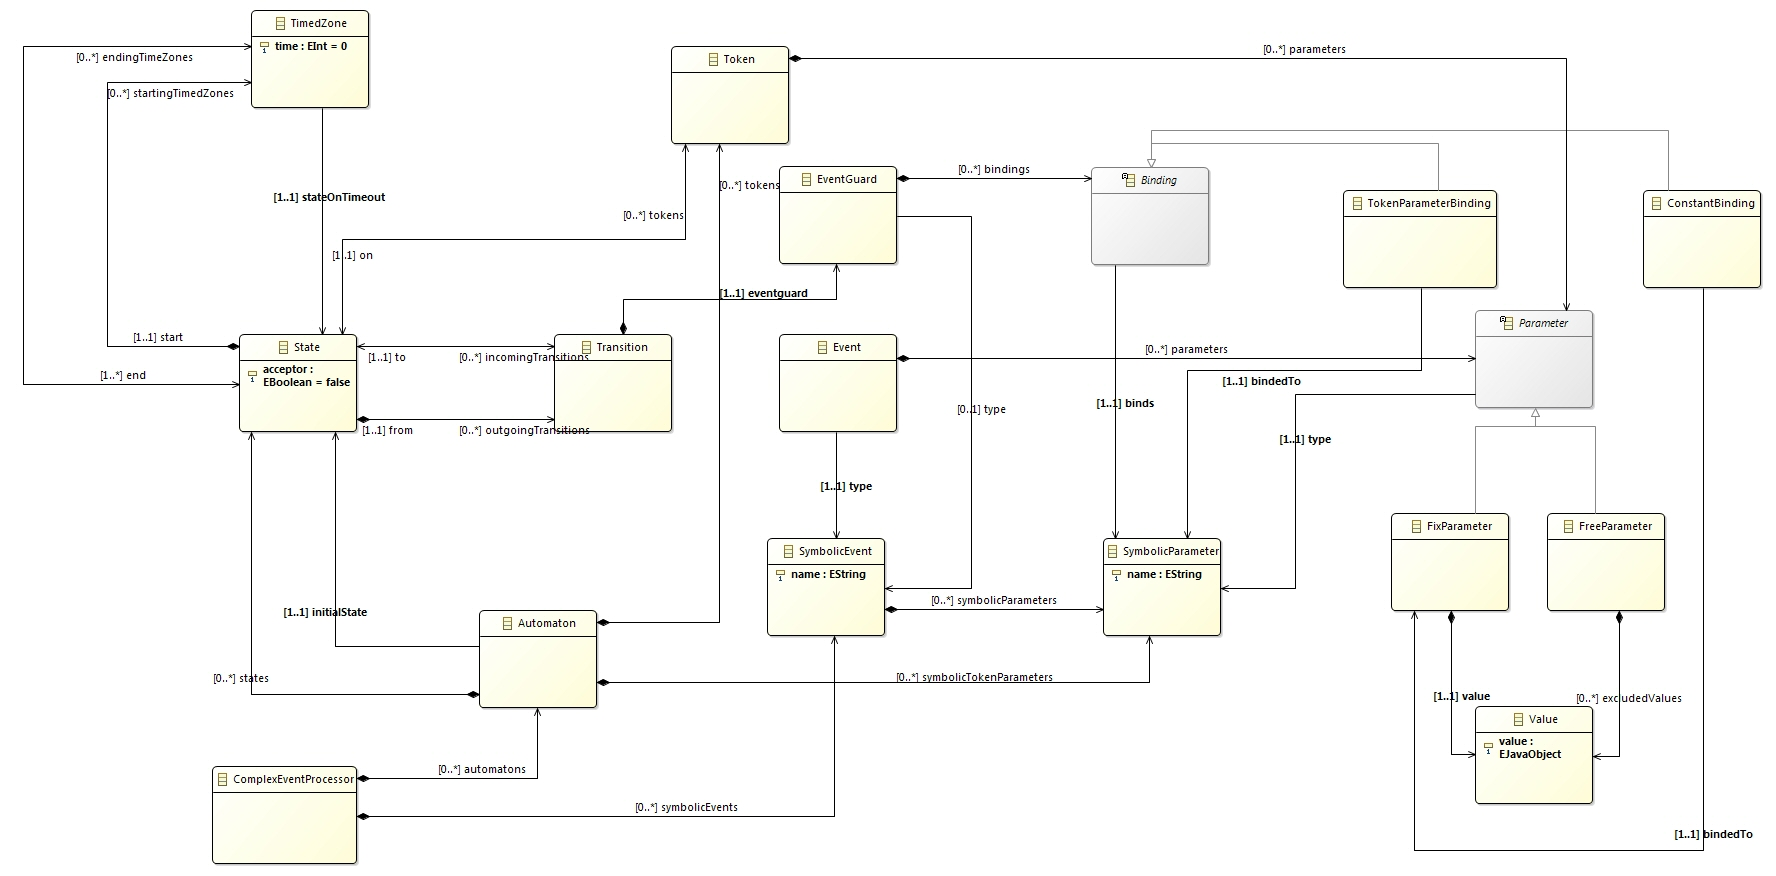
\includegraphics[width=0.9\linewidth]{include/figures/chapter_5/model}
			\caption{Automaton of the file example}
			\label{fig:cep:model}
			\end{figure}
		
			\subsubsection{Basic Automaton}
				The Event Automaton is represented with the State, Transition, and EventGuard classes.
				Every State has a boolean flag 
			\subsubsection{Timing}
			
			\subsubsection{Parameter}
			
			\subsubsection{Binding}
		
		\subsection{Executor}
			The algorithm first searches for all the activated transitions.
			If it finds an activated transition, it iterates over the tokens which are on the state. The first token with matching (non-confronting)
			parameter list will be split to the next state if there are new parameter bindings from the event, or moved if there are no new bindings.
			If a token enters an acceptor state it'll 
			next state 
